\chapter{\label{ch:ch01}ОБЗОР ПРОГРАММНЫХ СРЕДСТВ} % Нужно сделать главу в содержании заглавными буквами


\section{\label{subsec:ch01/sec01/sub01}Описание языка Python}

Python~\cite{python} - это высокоуровневый интерпретируемый язык программирования, который отличается простотой и понятностью синтаксиса. Он поддерживает различные парадигмы программирования, включая процедурное, объектно-ориентированное и функциональное программирование.

Python используется для разработки веб-приложений, научных вычислений, анализа данных, искусственного интеллекта, машинного обучения и других областей. Он имеет обширную стандартную библиотеку, которая включает в себя модули для работы с различными типами данных, сетевыми протоколами, графикой и д.р.

Python поддерживает динамическую типизацию и автоматическое управление памятью, что упрощает процесс разработки и делает его более гибким. Кроме того, Python является кроссплатформенным языком, что означает, что программы, написанные на нем, могут быть запущены на различных операционных системах без изменений.

В этом курсовом проекте Python будет использовано в связке с его модулем PyQT для создание игры "2048"

\section{\label{subsec:ch01/sec01/sub01}Описание библиотеки PyQT~\cite{РуковотствоPyQt5}  и библиотеки Random}
Описание библиотеки 
PyQT~\cite{PyQt} - это набор библиотек для разработки графических пользовательских интерфейсов (GUI) на языке программирования Python. Она предоставляет доступ к функциональности библиотеки Qt, которая является одной из самых популярных и мощных библиотек для создания GUI.

Основные особенности PyQT:
\begin{enumerate}
\item Кроссплатформенность: PyQT поддерживает работу на различных операционных системах, таких как Windows, macOS и Linux.
\item Обширный набор виджетов: PyQT предоставляет широкий выбор готовых виджетов для создания интерфейсов, таких как кнопки, текстовые поля, таблицы и многое другое.
\item Графический дизайн: с помощью PyQT можно легко создавать стильные и современные пользовательские интерфейсы с использованием каскадных таблиц стилей (CSS).
\item  Событийная модель: PyQT обладает мощной системой обработки событий, что позволяет реагировать на действия пользователя, такие как нажатия клавиш, перемещения мыши и т.д.
\end{enumerate}
Описание библиотеки Random
Библиотека random в Python предоставляет широкий спектр функций для работы с случайными числами. Она может использоваться для генерации случайных чисел, выбора случайных элементов из последовательностей, перемешивания данных и других операций, связанных со случайностью.

Вот некоторые из основных функций, которые можно использовать с помощью этой библиотеки:
\begin{enumerate}
\item  random.random(): Возвращает случайное число с плавающей точкой в интервале [0.0, 1.0).

\item  random.randint(a, b): Возвращает случайное целое число в диапазоне от a до b включительно.

\item  random.choice(seq): Выбирает случайный элемент из последовательности seq.

\item random.shuffle(seq): Перемешивает элементы последовательности seq в случайном порядке.

\item random.sample(population, k): Возвращает список уникальных элементов длиной k из последовательности population.
\end{enumerate}
Она  также предоставляет множество других функций для генерации случайных чисел и обработки данных.Помимо этого, библиотека random также предлагает возможность управления генератором псевдослучайных чисел, настройку начального состояния генератора и другие функции для работы с случайными данными.
\section{\label{subsec:ch01/sec01/sub01}Описание Qt Designer}
Qt Designer~\cite{QtDesigner} — это инструмент, предназначенный для создания графических пользовательских интерфейсов (GUI) на основе фреймворка Qt. Его основной целью является упрощение процесса разработки интерфейсов, позволяя разработчикам сосредоточиться на дизайне и функциональности, а не на написании большого количества кода.
\begin{enumerate}
\item Основные возможности Qt Designer:
\end{enumerate}
\begin{enumerate}
\item  Редактирование свойств виджетов:Каждый виджет имеет множество свойств, которые можно редактировать напрямую в Qt Designer. Это позволяет легко настраивать внешний вид и поведение каждого элемента интерфейса.

\item  Создание и управление компоновкой:Qt Designer поддерживает сложные схемы компоновки, что позволяет создавать адаптивные и динамические интерфейсы, которые корректно отображаются на различных экранах и в разных окнах.

\item  Поддержка сигналов и слотов:Qt Designer позволяет задавать соединения между сигналами и слотами для виджетов, что упрощает создание интерактивных элементов интерфейса.

\item Экспорт в XML (формат .ui):Разработанный интерфейс сохраняется в виде файла XML с расширением .ui, который можно использовать в дальнейшем для генерации кода на различных языках программирования.
\end{enumerate}
В своем проекте я использовал Qt Designer чтобы создать интерфейс игры 2048 и преобразовывал ее в код на языке програмирования пайтон.
\section{\label{subsec:ch01/sec01/sub01}Парадигмы програмирования }
 Существует несколько парадигм программирования, каждая из которых представляет собой различный подход к проектированию программного обеспечения. Каждая парадигма имеет свои преимущества и недостатки, и выбор парадигмы зависит от требований проекта и личных предпочтений разработчика.

Парадигмы программирования:
\begin{enumerate}
    \item Процедурное программирование --- парадигма, в которой программа разбивается на отдельные процедуры, которые могут быть вызваны из других частей программы. Эта парадигма часто используется для написания небольших программ, где не требуется много взаимодействия между различными частями программы;
    \item Объектно-ориентированное программирование (ООП)~\cite{b10} --- парадигма, в которой программа строится на основе объектов, которые являются экземплярами классов. Каждый объект имеет свои свойства и методы, которые могут быть использованы для взаимодействия с другими объектами. ООП широко используется в разработке больших и сложных программных систем;
    \item Функциональное программирование --- парадигма, в которой программа состоит из функций, которые принимают аргументы и возвращают значения. Эта парадигма часто используется для написания алгоритмов и математических вычислений;
    \item Логическое программирование  --- парадигма, в которой программа состоит из правил и фактов, и система логического вывода используется для нахождения ответов на запросы. Эта парадигма часто используется для решения задач искусственного интеллекта и баз данных;
    \item Событийно-ориентированное программирование --- парадигма, в которой программа реагирует на события, которые происходят в системе. События могут быть инициированы пользователем, другими программами или самой системой. Эта парадигма часто используется для написания графических интерфейсов пользователя и приложений, которые работают в реальном времени;
    \item Аспектно-ориентированное программирование --- парадигма, в которой программа разбивается на аспекты, которые представляют собой модули, отвечающие за определенные сферы функциональности. Эта парадигма часто используется для улучшения модульности и переиспользования кода;
    \item Декларативное программирование --- парадигма, в которой программа описывает, что должно быть сделано, а не как это должно быть сделано. Эта парадигма часто используется для написания запросов к базам данных и обработки данных;
    \item Реактивное программирование --- парадигма, в которой программа реагирует на изменения входных данных и автоматически обновляет выходные данные. Эта парадигма часто используется для написания приложений, которые работают в реальном времени, таких как системы мониторинга и управления.
\end{enumerate}


\chapter{\label{ch:ch02}РЕАЛИЗАЦИЯ ИГРЫ <<2048>>} 

\section{\label{subsec:ch01/sec01/sub01}Правила игры 2048}
Оригинальная игра 2048~\cite{2048} — это логическая игра, в которой целью является объединение плиток с одинаковыми числами, чтобы достичь плитки с числом 2048. Правила оригинальной игры 2048 таковы:
\begin{itemize}
\item Игрок управляет игровым полем размером 4x4 клетки.
\item В начале игры на поле случайным образом появляются две плитки с числами 2 или 4.
\item Игрок может сдвигать все плитки на поле в одном из четырёх направлений (вверх, вниз, влево, вправо). Все плитки двигаются в выбранном направлении до тех пор, пока не встретят препятствие (другую плитку или границу поля).
\item Если при сдвиге две плитки с одинаковыми числами сталкиваются, они объединяются в одну плитку с суммой этих чисел.
\item После каждого хода на поле случайным образом появляется новая плитка с числом 2 или 4.
\item Цель игры — достичь плитки с числом 2048.
\item Игра заканчивается, если на поле нет доступных ходов (ни одно сдвижение плиток не приводит к изменению положения или объединению).
\end{itemize}
В моей игре, так же как и в оригинале, цель одинакова но есть различия. Различия правил моей игры 2048 таковы:
\begin{itemize}
\item По стандарту игрок управляет игровым полем размером 4x4 клетки но можно поменять режим на 6х6 или 5х3
\item Игрок может взаимодействовать с игровым полем с помощью стрелок в окне игры.
\item Выйграть можно при сборе плитки с номером 62.
\item  Игра заканчивается, если на поле нет доступных ходов  но увидомление об окончании игры нет.
\end{itemize}
\section{\label{subsec:ch01/sec01/sub01}Этапы разработки игры 2048}
Для разработки игры "2048 на Python с применением библиотеки PyQt5" был составлен следующий план разработки, разделённый на ключевые этапы:
\begin{itemize}
\item  Разработка игрового интерфейса: Создание визуального дизайна и пользовательского интерфейса с использованием библиотеки PyQt5 для реализации игры 2048. Включает разработку сетки 4x4 ,6х6 , 5х3, а также элементов для отображения чисел и текущего счета.

\item  Реализация игровой логики: Разработка основных механизмов игры, включая движение плиток, объединение чисел при столкновении одинаковых плиток, а также генерацию новых плиток на игровом поле после каждого хода.
\item  Тестирование игры: Проверка игры на наличие ошибок и багов, тестирование игрового процесса для обеспечения корректной работы всех игровых механизмов и справедливого игрового опыта.
\item Подготовка документации и презентационных материалов: Составление технической документации и разработка презентации продукта для демонстрации потенциальным заинтересованным сторонам.
\end{itemize}
\section{\label{subsec:ch01/sec01/sub01}Разработка игрового интерфейса 2048}
Разработка игрового интерфейса – ключевой аспект в создании игры, который напрямую влияет на восприятие и опыт пользователя. Для игры “2048”, интерфейс должен быть не только визуально приемлемым , но и функциональным, чтобы поддерживать интерес игрока.
В моей игре нет главного меню,с запуска игры открывается окно игры в режиме 4х4.


\begin{figure}[ht]
    \centering
    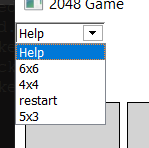
\includegraphics[width=0.5\textwidth]{images/2.png}
    \caption{Выподаюший список}
    \label{fig:enter-label}
\end{figure}
Главное меню игры “2048” представляет не хитрый интерфейс , который включает в себя следующие пункты:
\begin{enumerate}
\item Игровое поле с стрелками управления в правой части.
\item Exit этот пункт позволяет пользователю закрыть игру. Он расположен нижней левой  части окна.
3.  Счетчик очков который показывает текущие очки.
\end{enumerate}

Окно включает в себя и выподающий список с кнопками:
\begin{enumerate}
\item  help кнопка с напоминанием о правилах игры.
\item  6х6 это кнопка открывает окно игры 2048 только в режиме 6х6 игрового поля.
\item  4х4 это кнопка нужна если вы хотите переключится на режим 4х4
\item restart кнопка для обновления игрового поля 
\item  5х3 кнопка которая запускает режим игры с не симметричным игровым полем.
\end{enumerate}
\begin{figure}[ht]
    \centering
    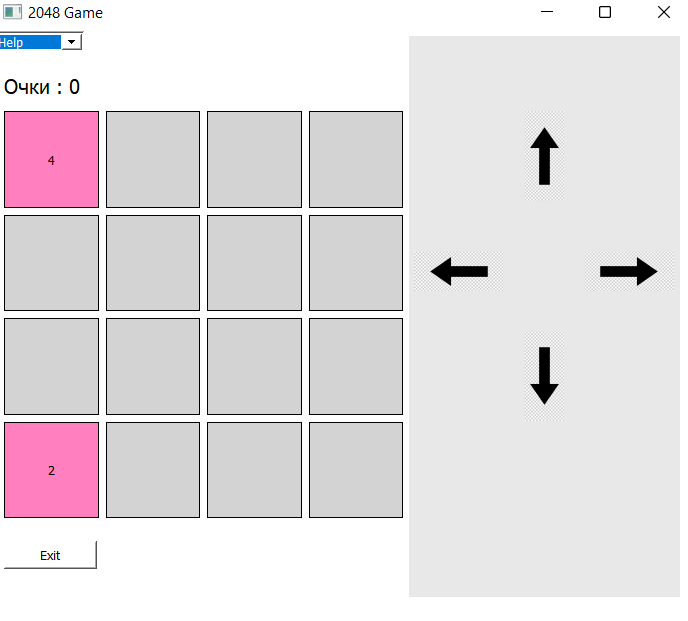
\includegraphics[width=0.5\textwidth]{images/1.png}
    \caption{основное игровое окно}
    \label{fig:enter-label}
\end{figure}
Игровогой процесс завязан на том что нужно собрать плитку с цифрой 2048.При выигрыше появляется окно с поздравлением и инструкциями как начать игру заново.
\begin{figure}[ht]
    \centering
    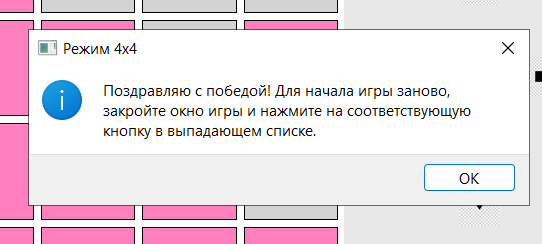
\includegraphics[width=0.5\textwidth]{images/3.png}
    \caption{Окно выигрыша}
    \label{fig:enter-label}
\end{figure}

При заполнении игрового поля и невозможности дальшейшего хода игра закончивается и при желании нужно начать заного с помошью кнопки в выподаюшем списке под названием restart.
\begin{figure}[ht]
    \centering
    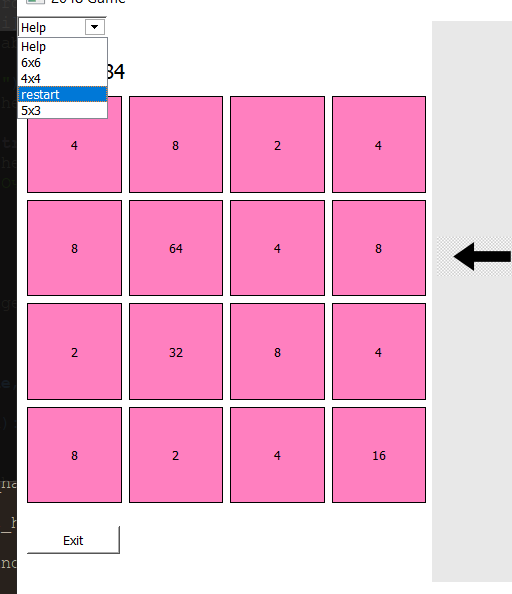
\includegraphics[width=0.5\textwidth]{images/4.png}
    \caption{кнопка restart}
    \label{fig:enter-label}
\end{figure}

Так же хочу показать чем отличается режимы 6х6х и 5х3 от режима 4х4.

\begin{figure}[ht]
    \centering
    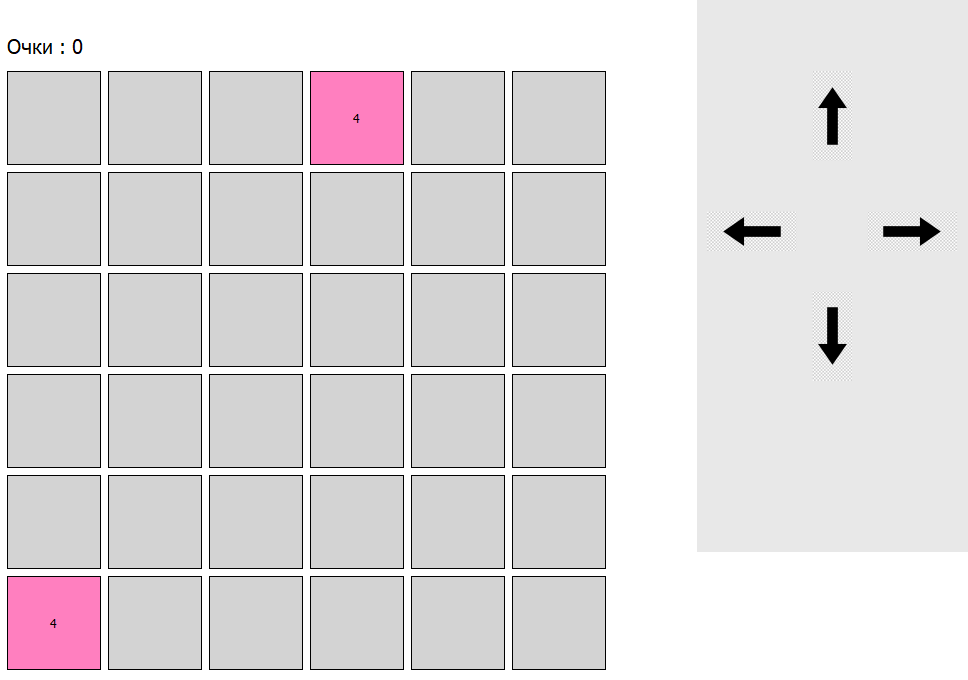
\includegraphics[width=0.5\textwidth]{images/5.png}
    \caption{Режим игры 6х6}
    \label{fig:enter-label}
\end{figure}
Режим игры 6х6 ни чем не отличается от режима 4х4 исключая размеры игрового поля.
\begin{figure}[ht]
    \centering
    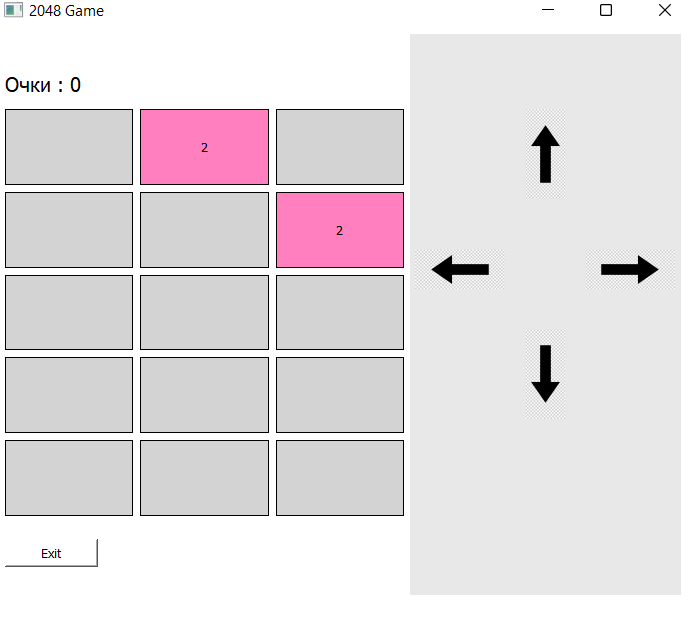
\includegraphics[width=0.5\textwidth]{images/6.png}
    \caption{Режим игры 5х3}
    \label{fig:enter-label}
\end{figure}
Аналогично режим игры 5х3 отличается только размером поля игры.




\section{\label{subsec:ch01/sec01/sub01}Реализация игрового процесса на примере режима 5х3}
Игра начинается с создания пустого игрового поля размером 5x3. 
    Создание игрового поля:
\begin{itemize}
\item Метод init\_game инициализирует доску и добавляет две случайные плитки (2 или 4) на пустые места.
\end{itemize}
Начальные настройки:
\begin{itemize}
\item Задаются начальные значения для счета (self.score) и размеры игрового поля (self.board\_size).
\end{itemize}
Добавление новых плиток
Выбор случайного места:
\begin{itemize}
\item Метод add\_random\_tile находит все пустые места на доске и случайным образом выбирает одно из них для размещения новой плитки.
\end{itemize}
Выбор значения плитки:
\begin{itemize}
\item На выбранное место добавляется плитка со значением 2 или 4, также выбранным случайным образом.
\end{itemize}
Обработка пользовательских вводов
Кнопки управления:
\begin{itemize}
\item В интерфейсе предусмотрены кнопки для перемещения плиток в четырех направлениях: вверх, вниз, влево и вправо.
\end{itemize}
Обработка движений:
\begin{itemize}
\item Метод handle\_move обрабатывает ввод пользователя, определяя направление движения плиток. В зависимости от направления вызывается соответствующий метод: move\_left\_handler, move\_right\_handler, move\_up\_handler или move\_down\_handler.
\end{itemize}
Перемещение и объединение плиток
Логика перемещения:
\begin{itemize}
\item Методы для обработки движений (например, move\_left\_handler) обрабатывают перемещения плиток в заданном направлении. Плитки сдвигаются в сторону и объединяются, если их значения совпадают.
\end{itemize}
Объединение плиток:
\begin{itemize}
\item Метод merge отвечает за объединение плиток. Если две соседние плитки движутся в одном направлении и имеют одинаковое значение, они объединяются, и значение удваивается.
Обновление интерфейса
\end{itemize}
Обновление состояния доски:
\begin{itemize}
\item Метод update\_ui обновляет интерфейс, отрисовывая текущее состояние игрового поля.
\end{itemize}
Обновление счета:
\begin{itemize}
\item Текущий счет отображается на экране и обновляется при каждом объединении плиток.
\end{itemize}
Проверка условий победы
Проверка победы:
\begin{itemize}
\item Метод check\_win\_condition проверяет, достигнуто ли значение плитки 32. Если да, отображается сообщение о победе.
\end{itemize}
Отображение сообщения о победе:
\begin{itemize}
\item Если условие победы выполнено, метод show\_win\_message отображает сообщение с поздравлением.
Завершение игры
\end{itemize}
Выход из игры:
\begin{itemize}
\item Кнопка "Exit" завершает игру и закрывает приложение.
\end{itemize}

\section{\label{subsec:ch01/sec01/sub01}Тестирование игры}
Тестирование игры 2048 на наличие каких либо не соответствий  и ошибок.
\begin{enumerate}
\item Тестирование соеденения плиток: Во время тестирование алгоритма на игровом поле режима 4х4, на ранних этапах разработки была выявлена ошибка не корректное слияние клеток(соеденялись числа которые не были одинаковы) связанная с тем что не правильно были написаны условия слияния чисел, после перерабоки условий такой ошибки замечено больше не было.Второй тест движения плиток:При сдвиге плиток в любом направлении (вверх, вниз, влево, вправо) корректно соединяются только одинаковые числа.

\item Тестирование кнопки выхода: После нажатия кнопки выхода окно с игрой закрылось.Кнопка работает карректно.
\item Тестирование кнопки в выподаюшем списке: Кнопка 6х6 работает корректно  и открывает окно игры с соответствующим игровым полем.
\item Тестирование кнопки в выподаюшем списке: Кнопка restart работает корректно  и  обнуляет игровое поле.
\item Тестирование кнопки в выподаюшем списке: Кнопка help работает корректно  и открывает окно где написаны правила игры.
\end{enumerate}    

\section{\label{subsec:ch01/sec01/sub01}Блок схема}
\begin{figure}[ht]
    \centering
    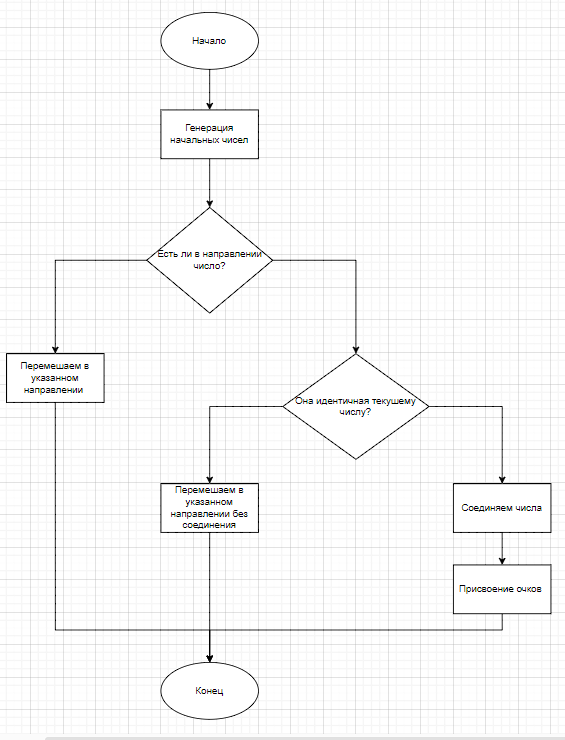
\includegraphics[width=0.7\textwidth]{images/7.png}
    \caption{Блок схема алгоритма игры 2048 }
    \label{fig:enter-label}
\end{figure}








